
\section{Alleles and genotypes}

\begin{frame}{Intended Learning Outcomes}

	\underline{Alleles and genotypes}

	\bigskip

        In this lecture you will learn
        \begin{itemize}
                \item to describe all different types of genetic data
                \item to demonstrate the mathematical relationship between allele and genotype frequencies
                \item to calculate inbreeding coefficients and test for deviation from Hardy-Weinberg Equilibrium from genomic data with \texttt{R}
        \end{itemize}

\end{frame}


\begin{frame}{Types of genetic data}

	Population genetics is applicable to all genetic \textit{variants} that can be distinguished by some means and that can be \textit{transmitted} from parents to offspring.

	\bigskip

	Any variants with these properties are called \textbf{alleles}:
	\begin{itemize}
		\item single nucleotide polymorphism,
		\item insertion/deletion,
		\item microsatellites.
	\end{itemize}

\end{frame}


\begin{frame}{Single nucleotide polymorphism (SNP)}

	\begin{figure}
        	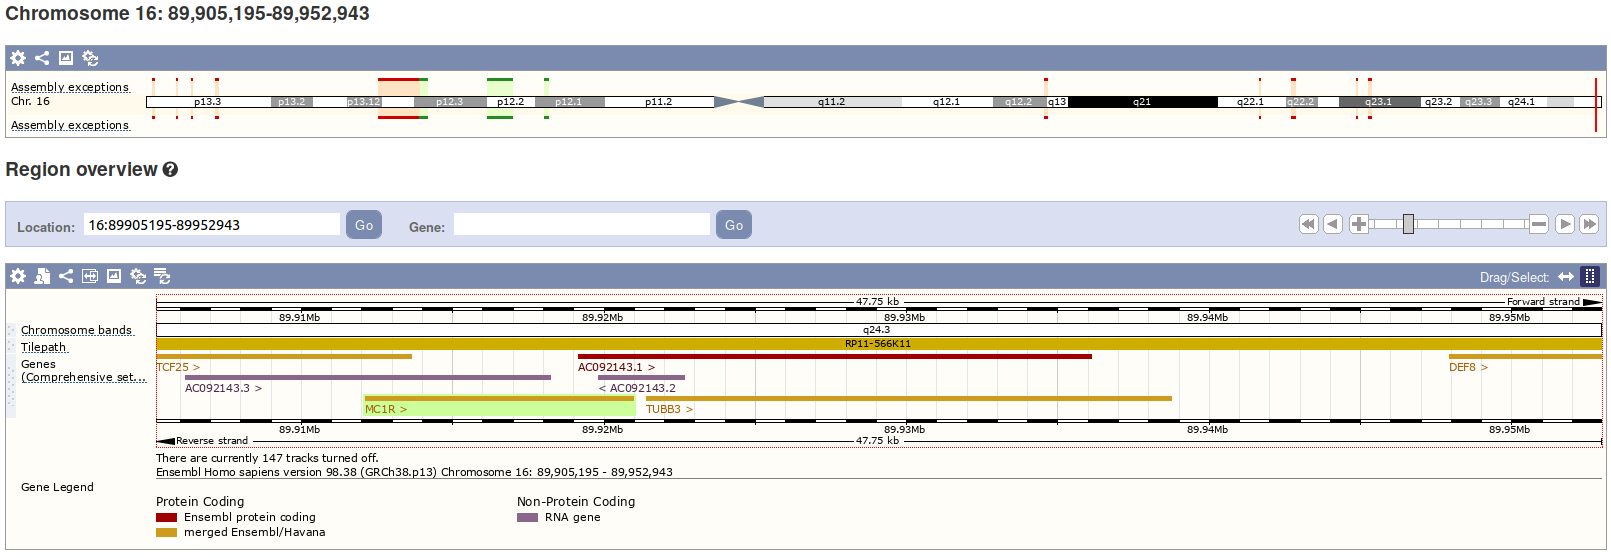
\includegraphics[width=0.9\textwidth]{Pics/MC1R} \
                \caption{\textit{MC1R} human gene}
        \end{figure}

	The \texttt{C/T} variation at position 478 in \textit{MC1R} is an example of a \textbf{single nucleotide polymorphism} (SNP, "snip").

\end{frame}


\begin{frame}{Single nucleotide polymorphism (SNP)}
	\bigskip

	\textit{MC1R} codes for a protein called melanocortin 1 receptor.

	\begin{columns}
		
		\column{0.5\textwidth}
        	
		\begin{figure}
                	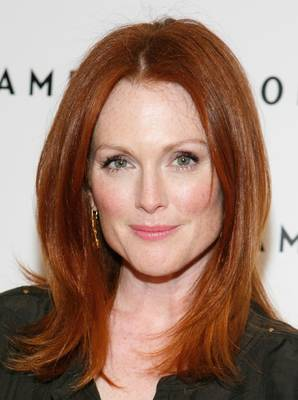
\includegraphics[width=0.6\textwidth]{Pics/red_hair} \
                	\caption{Julianne Moore}
        	\end{figure}

		\column{0.5\textwidth}

	        Individuals with two copies of \texttt{T} allele in position 478 of \textit{MC1R} 
		gene tend to have freckles and red hair.

		\bigskip

		This mutation disrupts the protein and causes an increase of the production 
		of red/yellow pigment melanin instead of brown/black.

	\end{columns}

\end{frame}


\begin{frame}{Insertion / deletion (indel)}
	\bigskip

	An \textbf{indel} is the insertion or deletion of few nucleotides.

 	\begin{columns}

                \column{0.4\textwidth}

                \begin{figure}
                        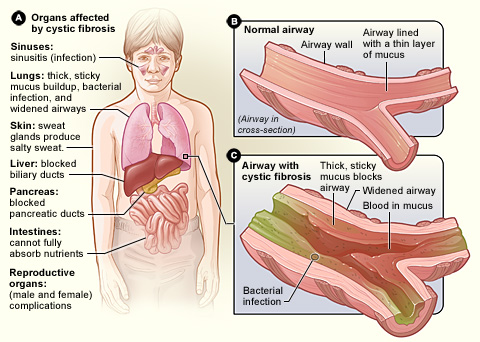
\includegraphics[width=1\textwidth]{Pics/cystic_fibrosis} \
                        \caption{Cystic fibrosis}
                \end{figure}

                \column{0.6\textwidth}

		\small

		\textit{CFTR} gene codes for a transmembrane protein involved in osmotic balance of cells.

		\bigskip

		Variant \texttt{$\Delta$F508} has a three-base deletion that results in the 
		absence of the 508th amino acid phenylanine (F).

                \bigskip

                This (genetically transmittable) mutation disrupts the protein and causes an 
		increase of the production of red/yellow pigment melanin.

        \end{columns}

\end{frame}


\begin{frame}{Microsatellites}
	\bigskip

	DNA replication machinery tends to miscopy repeated sequences in the genome.

	\begin{columns}
	
		\column{0.3\textwidth}

                \begin{figure}
                        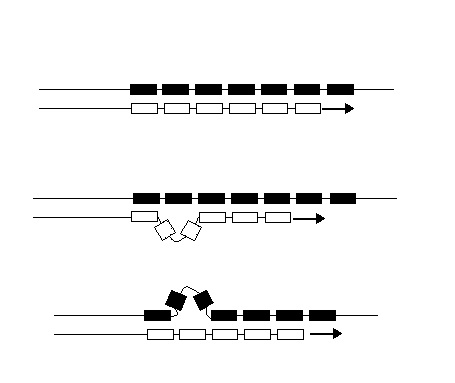
\includegraphics[width=1\textwidth]{Pics/microsat} \
                        \caption{DNA replication errors}
                \end{figure}

                \column{0.7\textwidth}

		\small{e.g. sequence \texttt{AGCTGCACACACACACACATGCTG} has \texttt{CA} motif 
	 	repeated seven times, while other individuals may have a different 
	 	number of copies, thus \texttt{(CA)$_n$}.}

		\bigskip

		Simple sequence repeats (SSRs) or \textbf{microsatellites} are variants on the number of
		repeats transmitted during meiosis, with a small possibility of error.

	\end{columns}

\end{frame}


\begin{frame}{Terminology}

        \bigskip

        \begin{itemize}
		\item allele: distinguishable and heritable (SNP, indel, microsat)
		\item locus: any position (or unit) in the genome with one or more alleles
		\item genotype: combination of alleles carried by an individual in a 
		particular locus
        \end{itemize}

	e.g. an individual has A and G alleles, and therefore has \texttt{AG} genotype, 
	at locus in position 8,789,654 of chromosome 1.


\end{frame}


\begin{frame}{Terminology}

 	\begin{figure}
        	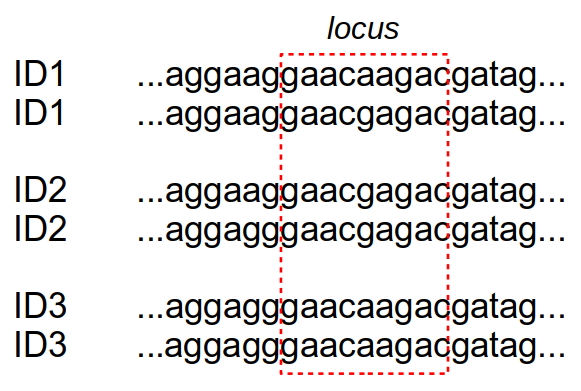
\includegraphics[width=0.6\textwidth]{Pics/locus} \
		\caption{A \textit{locus} of 20 base pairs (bp).}
        \end{figure}

\end{frame}


\begin{frame}{Terminology}

        \begin{figure}
                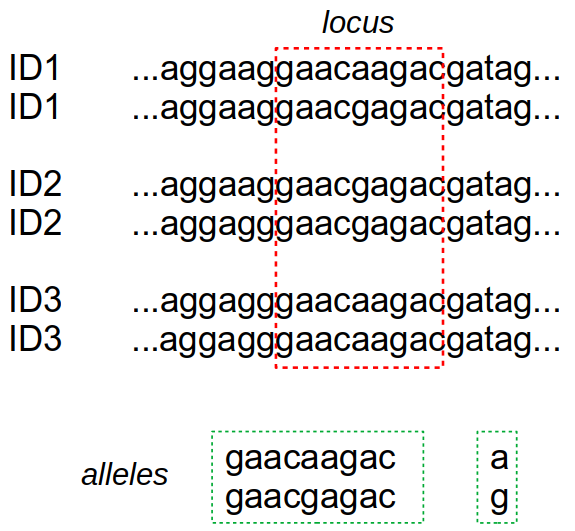
\includegraphics[width=0.6\textwidth]{Pics/alleles}
        \end{figure}

\end{frame}


\begin{frame}{Terminology}

        \begin{figure}
                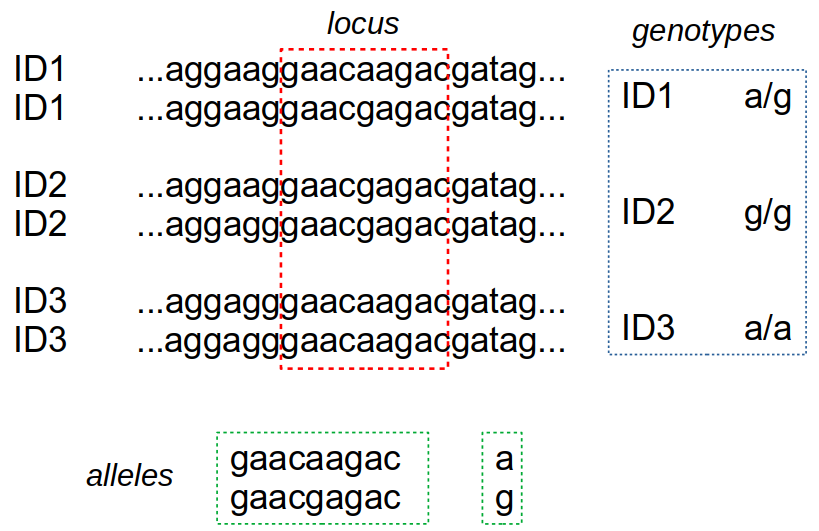
\includegraphics[width=0.8\textwidth]{Pics/genotypes}
        \end{figure}

\end{frame}


\begin{frame}{Terminology}

        \begin{figure}
                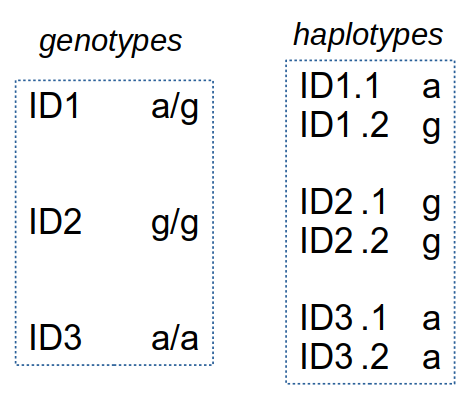
\includegraphics[width=0.6\textwidth]{Pics/haplotypes}
        \end{figure}

\end{frame}


\begin{frame}{Terminology}

	\bigskip

	As \textit{diploid} species have two copies of its chromosomes, for a collection of $N$
	diploid individuals, there are $2N$ gene copies at each locus, with one or more alleles.

	\bigskip

	As mutations are rare in most organisms, \textbf{di-allelic} models are often used, with 
	at most two alleles at each locus

	\bigskip

	e.g. at the red-hair \textit{vs.} non-red-hair locus in \textit{MC1R}, most individuals have C, 
	some have T but A and G haven't been observed suggesting a di-allelic model is a valid
	approximation here.

\end{frame}


\begin{frame}{Alleles and genotypes}

	\bigskip
	\small
	Population of $N=10$ individuals, $2N=20$ gene copies, and a total of 7 copies of allele $A$ 
	(yellow) and 13 copies of allele $a$ (blue)

 	\begin{columns}

                \column{0.4\textwidth}

                \begin{figure}
                        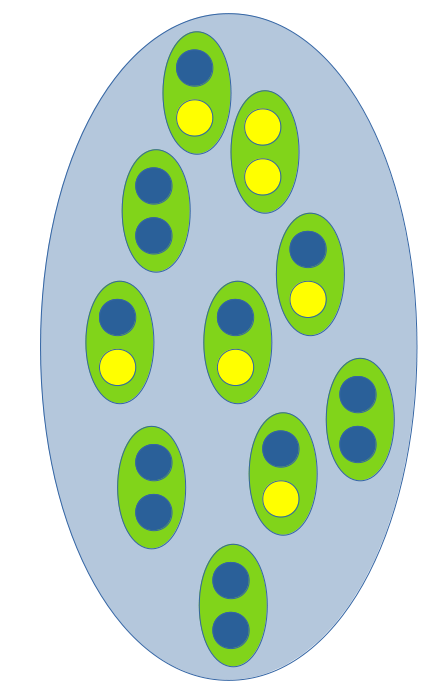
\includegraphics[width=0.8\textwidth]{Pics/population}
                \end{figure}

                \column{0.6\textwidth}

		What are the allele and genotype frequencies? \\
		\pause
		$f_A=$ \pause $7/20$ \\
		$f_a=13/20$ \\
		\vskip 0.5cm
		$f_{AA}=$ \pause $1/10$ \\
		$f_{Aa}=5/10$ \\
		$f_{aa}=4/10$ 
		
		\vskip 0.2cm
		$AA$ and $aa$ are homozygous individuals and $Aa$ are heterozygous individuals.

        \end{columns}

\end{frame}


\begin{frame}{Allele frequencies}

	\begin{columns}

                \column{0.4\textwidth}

                \begin{figure}
                        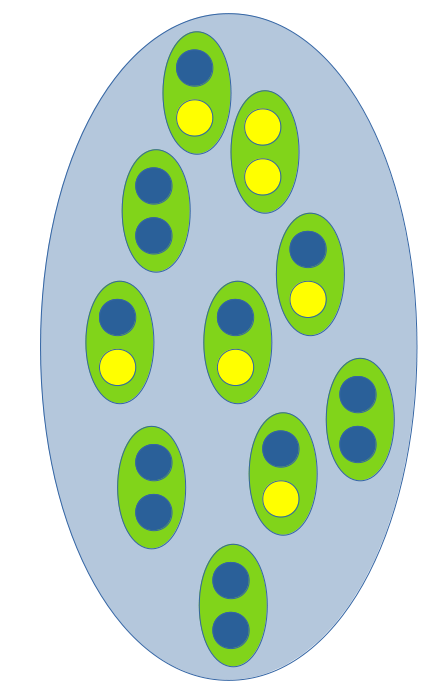
\includegraphics[width=0.8\textwidth]{Pics/population} \
                \end{figure}

                \column{0.6\textwidth}

		With $N$ diploid individuals and $A$ and $a$ alleles:

		\begin{equation}
			f_A = \frac{N_A}{2N}
		\end{equation}
		\begin{equation}
			f_a = \frac{N_a}{2N}
		\end{equation}

		where $N_A$ and $N_a$ are number of $A$ and $a$ alleles segregating in the 
		population, respectively.

		\bigskip

		Note that $f_A + f_a = 1$.

        \end{columns}

\end{frame}


\begin{frame}{Allele frequencies}

	\bigskip
        \begin{columns}

                \column{0.4\textwidth}

                \begin{figure}
                        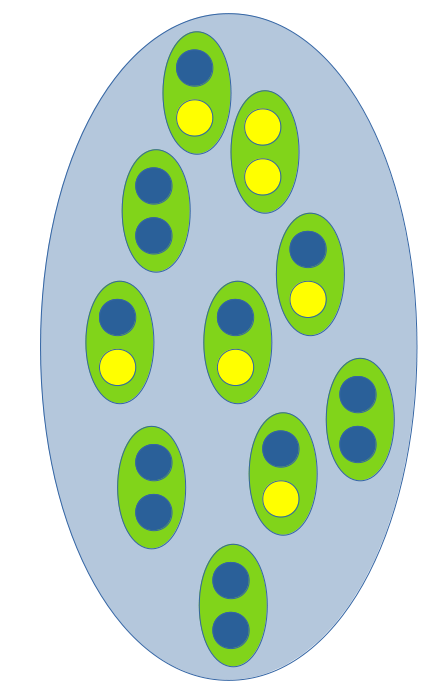
\includegraphics[width=0.8\textwidth]{Pics/population} \
                \end{figure}

                \column{0.6\textwidth}

		\begin{block}{}
			Much population genetics focuses on describing the changes of $f_A$ and
			$f_a$ with time.
		\end{block}

		\bigskip
		\small

		If we can describe how we expect allele frequencies to change through time in a population, 
		we have gained important insights of its evolution.

        \end{columns}


\end{frame}


\begin{frame}{Genotype frequencies}

        \begin{columns}

                \column{0.4\textwidth}

                \begin{figure}
                        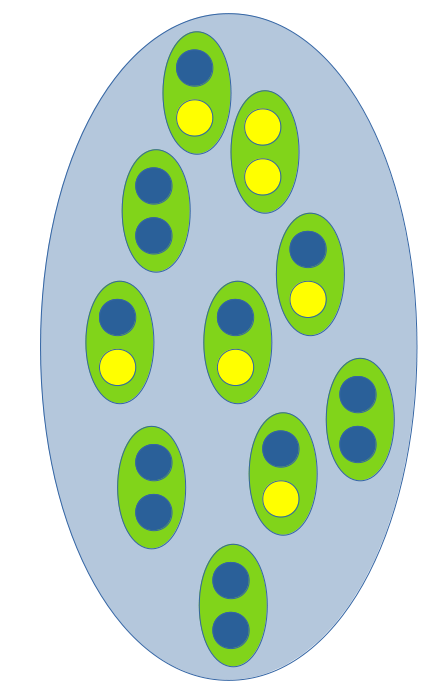
\includegraphics[width=0.8\textwidth]{Pics/population} \
                \end{figure}

                \column{0.6\textwidth}

		\small
		In a di-allelic locus there are three possible genotypes: $AA$, $Aa$ and $aa$.

                \begin{equation}
                        f_{AA} = \frac{N_{AA}}{N}
                \end{equation}
                \begin{equation}
                        f_{Aa} = \frac{N_{Aa}}{N}
                \end{equation}
		\begin{equation}
                        f_{aa} = \frac{N_{aa}}{N}
                \end{equation}

                \bigskip

                Note that $f_{AA} + f_{Aa} + f_{aa} = 1$.

        \end{columns}

\end{frame}

\begin{frame}{Allele and genotype frequencies}

        \begin{columns}

                \column{0.4\textwidth}

                \begin{figure}
                        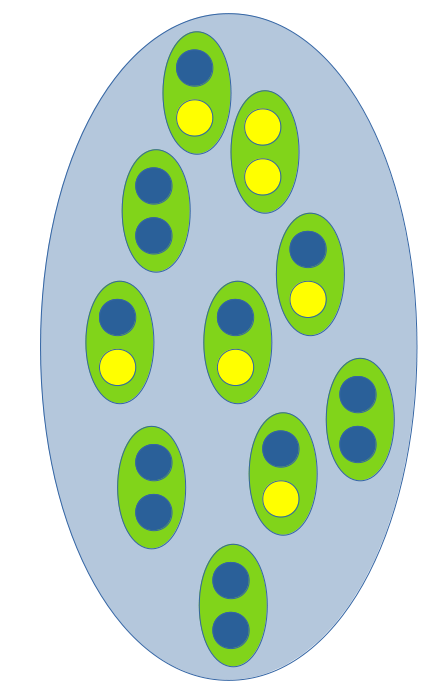
\includegraphics[width=0.8\textwidth]{Pics/population} \
                \end{figure}

                \column{0.6\textwidth}

                \small
		Can you calculate allele frequencies from genotype frequencies?

                \begin{equation}
                        f_A = \pause \frac{2N_{AA} + N_{Aa}}{2N} = f_{AA} + \frac{f_{Aa}}{2}
                \end{equation}

                \bigskip

                The proportion of heterozygous individuals in the population ($f_{Aa}$) is called
		the \textbf{heterozygosity}.
		\vskip 0.4cm
		The proportion of homozygotes ($1 - f_{Aa} = f_{AA} + f_{aa}$) is the \textbf{homozygosity} 
		of the population.

        \end{columns}

\end{frame}


\begin{frame}{\textit{MC1R} gene}

	\begin{figure}
                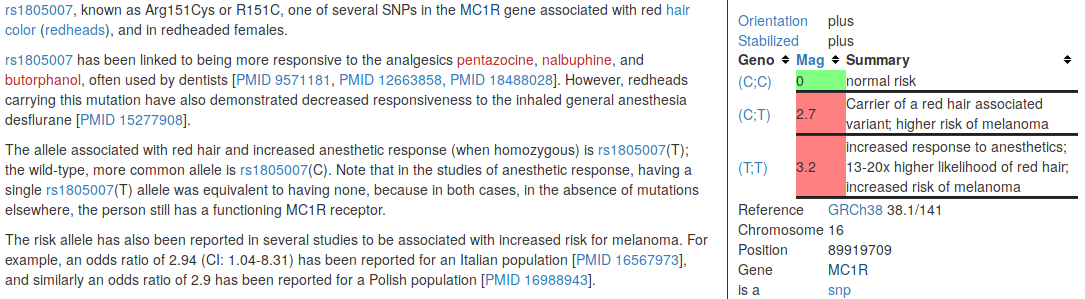
\includegraphics[width=1\textwidth]{Pics/mc1r_rs} \
                \caption{SNP associated to red hair with alleles C and T}
        \end{figure}

\end{frame}


\begin{frame}{\textit{MC1R} gene}

	Assume we obtain a \textit{random} sample of 30 individuals from the UK and find 25 individuals
	of genotype $CC$, 5 individuals with $CT$ and 0 with $TT$.

	\bigskip
	
	What are the \textit{estimated} genotype and allele frequencies?

	\pause
	\vskip 0.4cm
	$f_{CC}=25/30=0.833$, $f_{CT}=5/30=0.167$, $f_{TT}=0/30=0$ \\
	\pause
	\vskip 0.4cm
	$f_C=0.833+0.167/2=0.917$, $f_T=1-0.917=0.083$

	\vskip 0.4cm
	Why \textit{estimated}?

\end{frame}


\begin{frame}{Sample \textit{vs.} population}

	\begin{columns}

                \column{0.5\textwidth}

                \begin{figure}
                        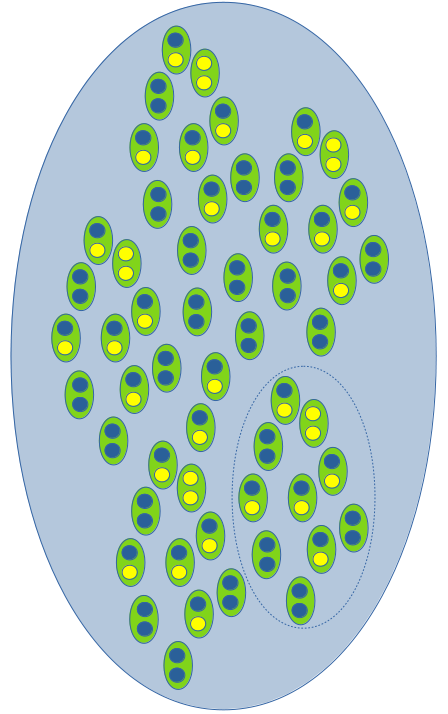
\includegraphics[width=0.6\textwidth]{Pics/sample} \
			 \caption{A random sample of individuals from a population}
                \end{figure}

                \column{0.5\textwidth}

		\small
		We cannot know the true genotype/allele frequency in the entire population 
		but we aim at estimating it from a random sample of individuals.
		\bigskip
		\begin{block}{}
			We calculate the sample allele frequency as a proxy for the unknown population allele frequency.
		\end{block}

	\end{columns}

\end{frame}


\begin{frame}{Alleles to genotypes}

	We can calculate allele frequencies from genotype frequencies.
	\begin{block}{}
		Can we \textit{predict} genotype frequencies from allele frequencies?
	\end{block}

	e.g. knowning that the frequency of $T$ in position 478 of the \textit{MC1R} gene is $0.08$, 
	what proportion of the population is expected to have genotype $TT$?

\end{frame}


\begin{frame}{Alleles to genotypes}

	\begin{figure}
        	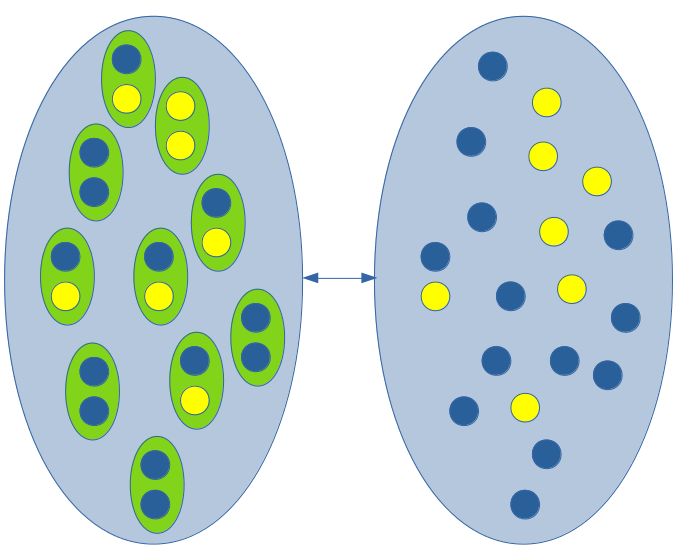
\includegraphics[width=0.6\textwidth]{Pics/alleles2geno}
        \end{figure}

\end{frame}


\begin{frame}{Alleles to genotypes}

        \begin{columns}

                \column{0.5\textwidth}

                \begin{figure}
                        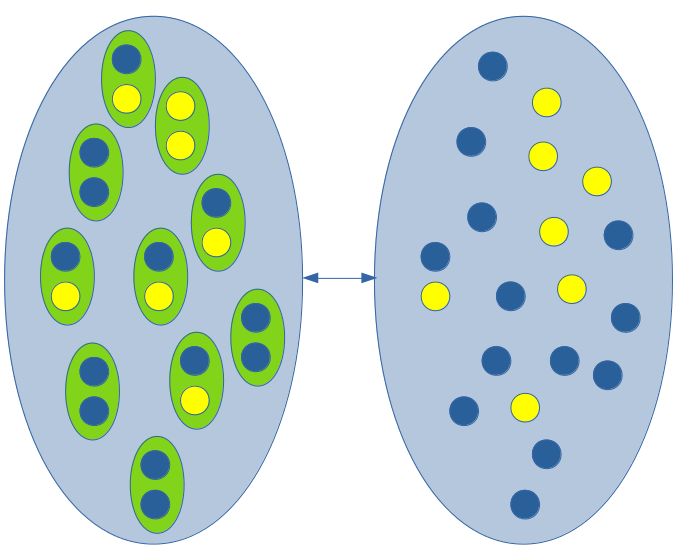
\includegraphics[width=0.8\textwidth]{Pics/alleles2geno}
                \end{figure}

                \column{0.5\textwidth}

                \small
                \begin{block}{Assumptions}
			\begin{itemize}
				\item random mating: individuals mate with each other without regard to genotype
				\item males and females have equal allele frequency
				\item di-allelic locus
			\end{itemize}
                \end{block}

        \end{columns}

\end{frame}


\begin{frame}{Hardy-Weinberg Equilibrium (HWE)}

	\begin{table}[h]
                \centering
                \begin{tabular}{p{0.2\textwidth} p{0.2\textwidth} p{0.2\textwidth} p{0.2\textwidth}}
                        \toprule
                        \multicolumn{2}{p{0.5\textwidth}}{Genotype frequencies under HWE} \\
                        \midrule
			Genotype & $AA$ & $Aa$ & $aa$ \\
			Frequency & $f_A^2$ & $2f_Af_a$ & $f_a^2$\\
                        \bottomrule
                \end{tabular}
        \end{table}

\end{frame}


\begin{frame}{Hardy-Weinberg Equilibrium (HWE)}

	\small
	\begin{itemize}
		\item expected homozygosity is $f_A^2 + f_a^2$
		\item expected heterozygosity is $2f_Af_a$
		\pause
		\item $f_A^2 + 2f_Af_a + f_a^2 = 1$
		\pause
		\item random mating does not change the allele frequencies in the next generation: \\
		$f'_A = f_A^2 + 2f_Af_a/2 = f_A^2 + 2f_A(1-f_A)/2=f_A$
	\end{itemize}

\end{frame}


\begin{frame}{HWE in \textit{MC1R}}

        \begin{columns}

                \column{0.5\textwidth}

                \begin{figure}
                        
\includegraphics[width=0.5\textwidth]{Pics/grint} \\
			\caption{Rupert Grint}
                \end{figure}

                \column{0.5\textwidth}

                \small
		With an allele frequency of $0.08$ for allele $T$ in the US population,
		how many $TT$ homozygotes might we expect?

		\pause
		It's $0.08^2=0.0064$.
		
		\bigskip

		Individuals with $TT$ genotype will likley have red hair, but a much larger
		proportion of the population has red hair. Why?

        \end{columns}

\end{frame}


\begin{frame}{Deviations from HWE}

        \begin{columns}

                \column{0.5\textwidth}

                \begin{figure}
                        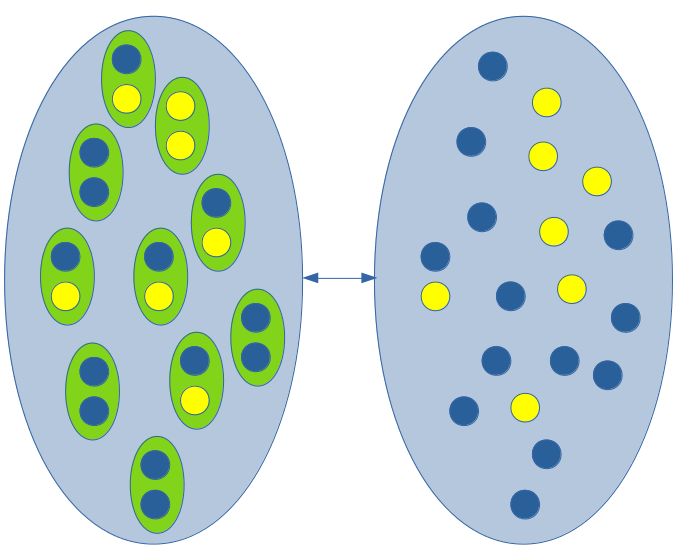
\includegraphics[width=0.8\textwidth]{Pics/alleles2geno}
                \end{figure}

                \column{0.5\textwidth}

                \small
                \begin{block}{Assumptions for HWE}
                        \begin{itemize}
                                \item random mating: individuals mate with each other without regard to genotype
				\item (males and females have equal allele frequency)
				\item (di-allelic locus)
                        \end{itemize}
                \end{block}

        \end{columns}

\end{frame}


\begin{frame}{Deviations from HWE}

	\small
	\begin{itemize}
		\item Assortative mating: not random with respect to genotype
		\pause
		\item Inbreeding: mating of related individuals
		\pause
		\item Population structure: sample of individuals from two or more subpopulations
	\end{itemize}

 	\begin{figure}
        	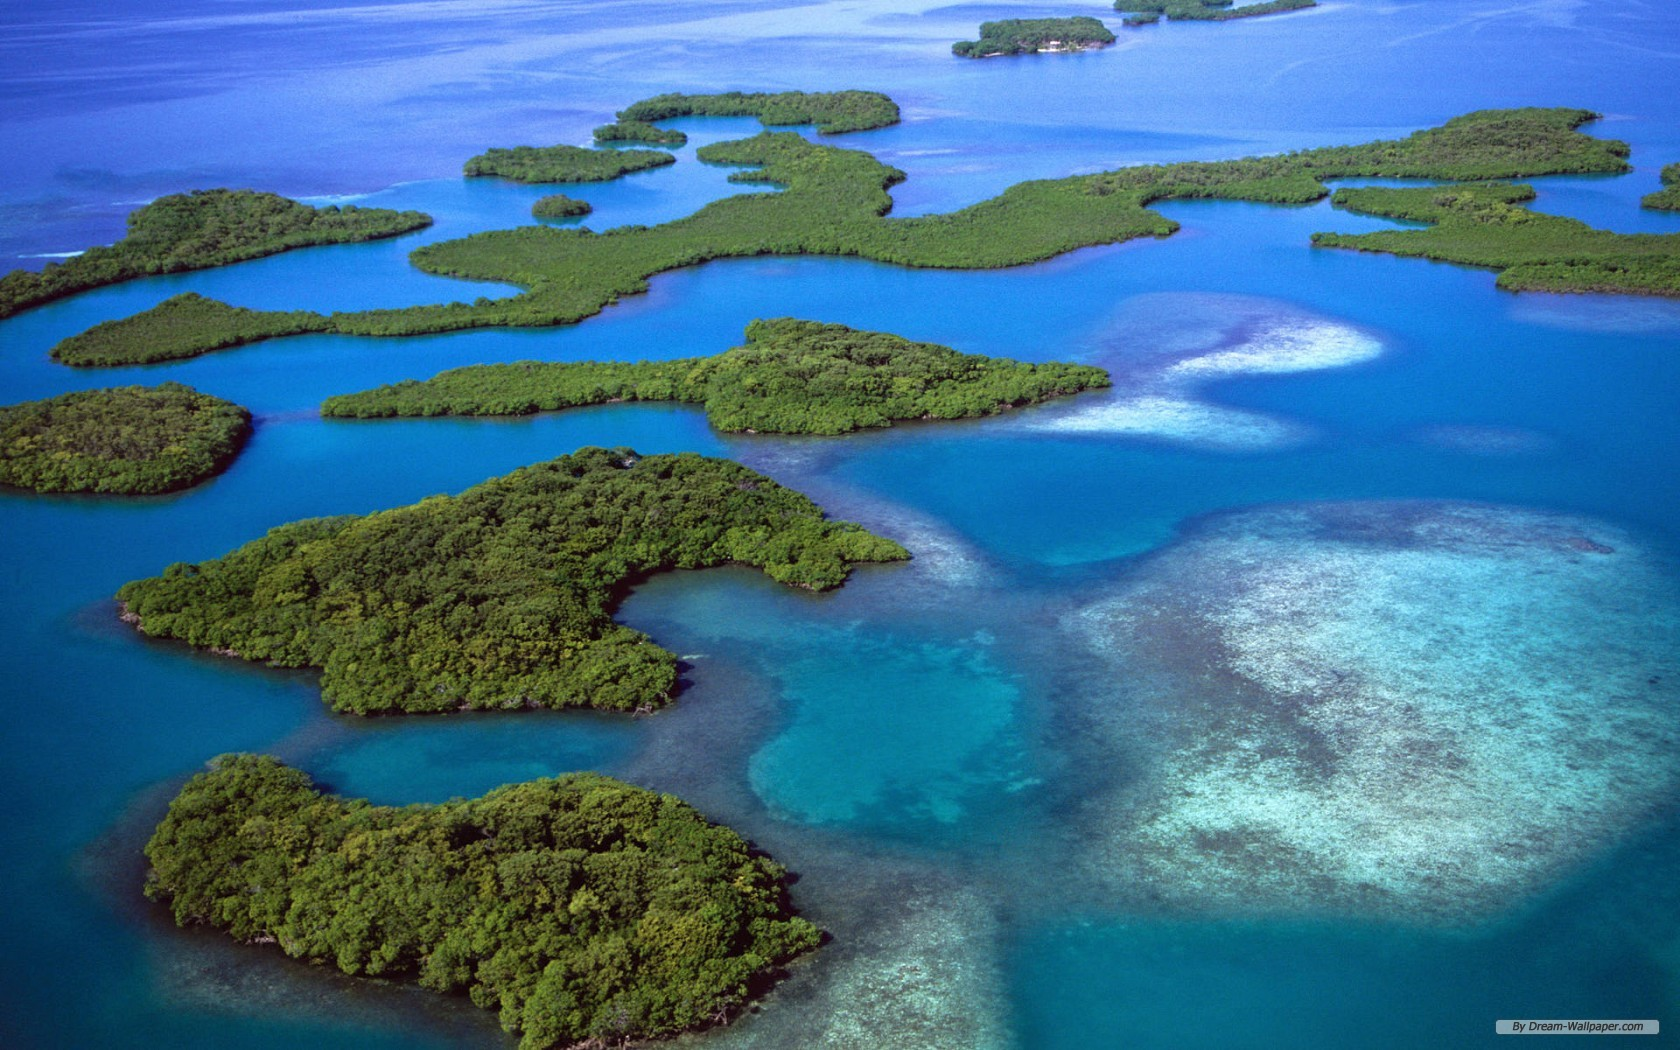
\includegraphics[width=0.4\textwidth]{Pics/galapagos}
        \end{figure}


\end{frame}


\begin{frame}{Population structure}

	\begin{columns}

                \column{0.5\textwidth}

                \begin{figure}
                        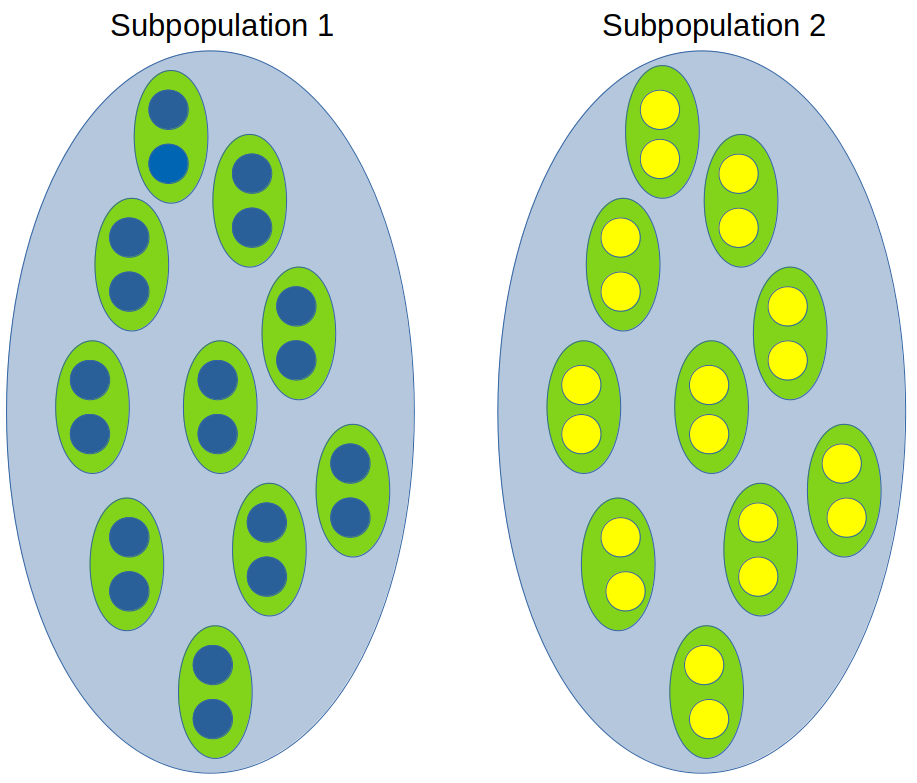
\includegraphics[width=1\textwidth]{Pics/structure}
                \end{figure}

                \column{0.5\textwidth}

                \small
                \begin{itemize}
                	\item population subdivision
                        \item continuous spatial distribution of individuals
                        \item migration from an unsampled population
			\item ...
                \end{itemize}

        \end{columns}

\end{frame}


\begin{frame}{Deviations from HWE}

        \small
        \begin{itemize}
                \item Assortative mating: not random with respect to genotype
                \item Inbreeding: mating of related individuals
                \item Population structure: sample of individuals from two or more subpopulations
		\item Natural selection
        \end{itemize}

	\begin{figure}
        	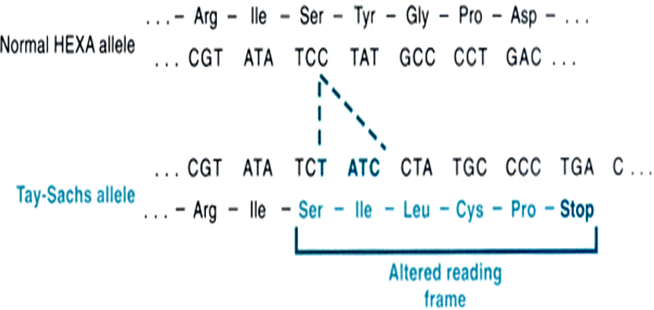
\includegraphics[width=0.5\textwidth]{Pics/tay} \\
		\caption{Insertion in \textit{HEXA} gene associated with Tay-Sachs disease}
        \end{figure}


\end{frame}


\begin{frame}{Inbreeding coefficient}

	\small
	\begin{block}{Inbreeding coefficient ($F$)}
		Most common statistic to measure deviations from HWE: it describes the degree to which heterozygosity
		is reduced both in individuals and in populations.
	\end{block}

	\begin{equation}
		F = \frac{2f_Af_a - f_{Aa}}{2f_Af_a}
	\end{equation}

	\bigskip

	If $F=0$ the population is in HWE, if $F=1$ \pause there are no heterozygotes.

\end{frame}


\begin{frame}{Inbreeding coefficient}

	\small
	\begin{equation}
		f_{Aa} = 2f_Af_a(1-F)
	\end{equation}

	\begin{itemize}
		\item The proportion of heterozygotes in the population is reduced by a factor of $F$ from that expected under HWE.
		\item If we know $F$ and the allele frequencies, we can predict genotype frequencies without assuming HWE.
	\end{itemize}

	Are there species likely to deviate from HWE?

\end{frame}


\begin{frame}{Self-fertilizing plants}

	\begin{columns}

                \column{0.5\textwidth}

                \begin{figure}
                        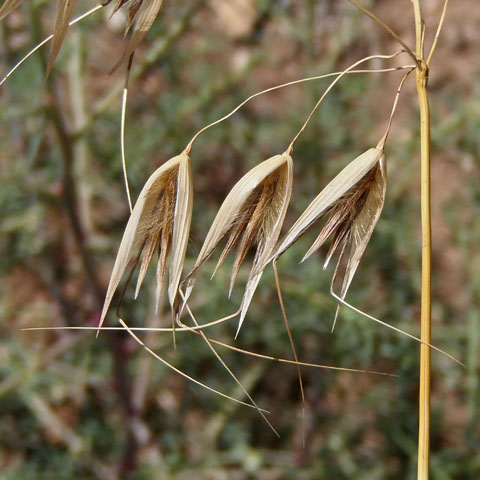
\includegraphics[width=0.8\textwidth]{Pics/avena} \\
			\caption{Flower of wild oats (\textit{Avena fatua})}
                \end{figure}

                \column{0.5\textwidth}
		\small

                Genotype frequencies at one locus are: \\
		$f_{AA}=0.58$, $f_{Aa}=0.07$, $f_{aa}=0.35$.

		\begin{enumerate}
			\item What is $F$, the inbreeding coefficient?\\
			\pause
			$f_A=0.58 + 0.07/2=0.615$, $f_a=1-0.615=0.385$ \\
			$F = (2 \times 0.385 \times 0.615 - 0.07) / (2 \times 0.385 \times 0.615) = 0.852$
			\item Does it deviate from HWE?
		\end{enumerate}
		
        \end{columns}


\end{frame}


\begin{frame}{Testing for deviations from HWE}

	\begin{columns}

                \column{0.3\textwidth}

                \begin{figure}
                        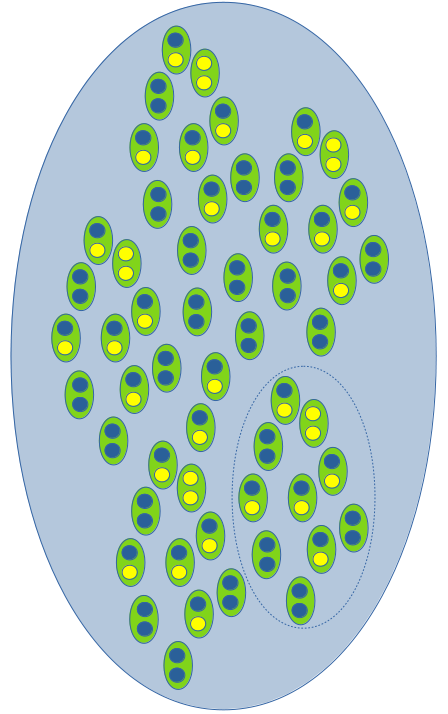
\includegraphics[width=0.9\textwidth]{Pics/sample}
                \end{figure}

                \column{0.7\textwidth}

                \small
                \begin{itemize}
			\item A random sample for a population in HWE may deviate from HWE.
			\item We need a formal statistical test: \\
			\vskip 0.4cm
			Null hypothesis: genotype frequencies follow those predicted by HWE \\
			\vskip 0.2cm
			Alternative hypothesis: genotype frequencies do \textbf{not} follow those predicted by HWE
                \end{itemize}

        \end{columns}

\end{frame}


\begin{frame}{Testing for deviations from HWE}

	Chi-square test: $\chi^2 = \sum_{i=1}^k \frac{(E_i - O_i)^2}{E_i}$

	\begin{itemize}
		\item observed values ($O_i$, genotype frequencies)
		\item expected values ($E_i$, expected genotype frequencies under HWE)
		\item degrees of freedom: $3-1-1=1$
	\end{itemize}

	\bigskip

        If $\chi^2$ is large enough, we reject the null hypothesis.

\end{frame}


\begin{frame}{Testing for deviations from HWE}

	\small
        $\chi^2 = \sum_{i=1}^k \frac{(E_i - O_i)^2}{E_i}$
	\bigskip
	e.g. observed genotypes: $O_{AA}=20$, $O_{Aa}=10$, $O_{aa}=10$ 

	\begin{itemize}
		\pause
		\item $f_{AA}=1/2$, $f_{Aa}=1/4$, $f_{aa}=1/4$
		\pause
		\item $f_A=1/2 + (1/4)/2 = 5/8$, $f_a=1/4 + (1/4)/2=3/8$
		\pause
		\item $E_{AA}=40 \times (5/8)^2 = 15.625$, $E_{Aa}=40 \times 2 \times 3/8 \times 5/8=18.75$, $E_{aa}=40 \times (3/8)^2 = 5.625$
		\item
		$\chi^2 = ... + ... + ... = 8.711$
	\end{itemize}

	Is $8.711$ "large enough"?

\end{frame}


\begin{frame}{Testing for deviations from HWE}

	\small

	We need to compare our valye $8.711$ with a critical value for a chi-square distribution with one degree of freedom.

	\begin{table}
	\begin{tabular}{c|c|c|c|c|c|c|c|c|c}
	\toprule
	d.f & .995 & .99 & .975 & .95 & .9 & .1 & .05 & 0.025 & 0.1\\
	\midrule
	0 & 0 & 0 & 0 & & 0.02 & 2.71 & 3.84 & 5.02 & 6.63\\
	\bottomrule
	\end{tabular}
	\end{table}

	Do we reject the null hypothesis of HWE?
	\pause

	Yes, since \textit{p}-value is $<0.05$, assuming such threshold for significance (but remember that statistical significance does NOT imply biological significance).

\end{frame}


\begin{frame}{Intended Learning Outcomes}

	\underline{Alleles and genotypes}

        \bigskip

	In this lecture you have learnt
	\begin{itemize}
		\item to describe all different types of genetic data
		\item to demonstrate the mathematical relationship between allele and genotype frequencies
		\item to calculate inbreeding coefficients and test for deviation from 
		Hardy-Weinberg Equilibrium from genomic data using \texttt{R}
	\end{itemize}

\end{frame}




